\startchapter{Software Implementation}
\label{chapter:implementation}
\section{Introduction}
The \acrfull{IC} life-cycle was introduced in section~\ref{sec:methodology}.
It is the process where \acrshort{IC}s begin as ideas and end as products to be sold.
The process is expensive, delicate, and consumes thousands of man hours.
To streamline this process and minimize risk the industry is more frequently relying on third-party sources for a variety of steps~\cite{thirdPartyLogistics}. 
For manufacturers it is imperative to ensure that their products are not at risk while in the hands of these outsourced services. 
Conversely, it is undesirable for the the required security and quality assurance measures to mitigate the benefit gained by using these services. 

The \NameNoPeriod can provide manufacturers additional security that takes only minutes to complete; the analysis requires only a few button clicks.
It was built to be a stand-alone application.
Manufacturers and researchers alike are already required to purchase large and expensive pieces of equipment; much of which requires arduous installation and configuration.
The \NameNoPeriod is light-weight, cross platform and does not require installation.
Its application can greatly improve security at little to no cost.

\section{Technologies Used}
\subsection{\Xilinx}
\Xilinx is one of the two largest manufacturers of \acrshort{FPGA}s; their devices are considerably more popular than their competitors.
The configuration of devices employs a well known series of steps referred to as the \Xilinx ``tool-chain''~\cite{xilnxDevManual}.
The ``tool-chain'' not only compiles user designs and constraints into the configuration \gls{Bitstream} but performs a series of complex operations to optimize designs and effectively implement them on any \Xilinx model of the user's choosing.
\begin{enumerate}
	\item \textbf{\gls{sch2hdl}}: \glsdesc{sch2hdl}
	\item \textbf{\gls{XST}}: \glsdesc{XST}
	\item \textbf{\gls{MAP}}: \glsdesc{MAP}
	\item \textbf{\gls{PAR}}: \glsdesc{PAR}
	\item \textbf{\gls{ngdbuild}}: \glsdesc{ngdbuild}
	\item \textbf{\gls{trce}}: \glsdesc{trce}
	\item \textbf{\gls{Bitgen}}: \glsdesc{Bitgen}
\end{enumerate}
Each step produces a series of files that are used for a variety of purposes. 
Often the resultant files are used by the subsequent step but some are intended for user information.
The \gls{ngdbuild} tool generates what is known as the netlist for the design.
The netlist is a description of the connectivity of the circuit implemented on the device. 
The generated netlist is in a non human-readable format in an ``ndc'' file.
Fortunately, \Xilinx provides an additional tool called \gls{xdl2ndc} which allows the conversion to the human-readable \acrfull{XDL}.
\subsubsection{\acrfull{XDL}} \label{sec:XDL}
The \acrfull{XDL} is a human-readable ASCII format; though it is not actively part of the ``tool-chain'' it is considered a native netlist format for describing and representing \acrshort{FPGA} designs~\cite{xdlTutorial}. 
In a netlist, a ``part'' is a human-defined component which is to be implemented.
Netlists either contain or refer to descriptions of the parts used and where in the device they are implemented.
When a part is used it is called an ``instance''; thus each ``instance'' has a definition, sometimes referred to as a master.

An \acrshort{XDL} file contains two sections, the instance placement and configuration section, and the net routing section. 
The placement and configuration section provides a list of every instance in a design. 
Their descriptions include all of the configuration details required for their implementation on a component (power settings, logic, timing configurations... etc).
In the \Xilinx jargon, a net refers to any electrical path between two components; more specifically, a net describes a communication channel.
The gate-array of a \Xilinx device is composed of a grid of wires.
These wires can be fused together by \acrfull{PIP} to make a useful connection between two components, thus creating a net.
The output-pin of a net receives the signal from the transmitting component while the input-pin delivers the signal to the corresponding receiver.
The \acrshort{PIP}s in-between the end-points dictate the path the signal takes between the two components.
The net routing section of the \acrshort{XDL} file describes every path in the design.
Combined, these two sections completely describe a design and how it is implemented.
The information provided by the \acrshort{XDL} file is used by the \NameNoPeriod to relate any of the effects of a discovered trojan to the user's intended operation. 
\subsubsection{XDLRC} \label{sec:XDLRC}
The \acrshort{XDL} file describes the design implemented on a device.
From this a lot of information regarding the composition of a \Xilinx device can be learned but it does not provide the entire description; only what has been used by the design.
The \gls{xdl2ndc} command line tool provides an option to generate a resource report file referred to as an XDLRC file. 
A XDLRC file describes the entire architecture of a \Xilinx \acrshort{FPGA}.

\ConditionSize
\begin{lstlisting}[label={lst:xdlrc}, language=Python, caption={A hierarchical XDLRC resource description of a Spartan 6 FPGA consisting of a header, a tile section, and a trailing device summary~\cite{xdlTutorial}}]
#Header section
(xdl_resource_report v0.2 xc6slx16csg324-3 spartan6
# Device Level Dimensions
(tiles 73 62
...
	#Configurable logic block with two slices
	(tile 4 6 CLEXL_X1Y61 CLEXL 2
		(primitive_site SLICE_X0Y61 SLICEL internal 45
			(pinwire A1 input L_A1)
		...
		(primitive_site SLICE_X1Y61 SLICEX internal 43
		...
		(pinwire D output XX_D)
	...)
	# Interconnect tile
	(tile 4 5 INT_X1Y61 INT 1
	...
		(wire EE2B0 2
			(conn CLEXM_X2Y61 CLEXM_EE2M0)
			(conn INT_BRAM_X3Y61 EE2E0)
		...
		# Programmable Interconnect Points
		(pip INT_X1Y61 EE2E0 -> EE2B0)
		(pip INT_X1Y61 EE4E0 -> EE2B0)
		(pip INT_X1Y61 EL1E_S0 -> LOGICIN_B9)
	...)
# summary
(summary tiles=4526 sites=5378 sitedefs=46 numpins=157962 numpips=5782505))
\end{lstlisting}
\normalsize

Listing~\ref{lst:xdlrc} provides an example of the XDLRC format.
The report begins with a header describing the device.
It then reports that the overall architecture contains a matrix of tiles, 73-wide and 62-tall.
Further down is a configurable logic block at coordinate (4,6) and an interconnect tile at coordinate (4,5).
Each of these tile descriptions provide details of the subcomponents they contain, pinwires, \acrshort{PIP}s, slices...etc.
The \gls{xdl2ndc} tool is capable of generating a variety of different XDLRC files for a device, ranging in the level of detail.
The smaller files can be around 10MB while the fully detailed descriptions can reach 7GB in size.
\subsection{Java} \label{sec:java}
Java is a powerful and general-purpose programming language. 
It is specifically designed to be as independent as possible.
The original developer, James Gosling, intended the language to allow developers a comfortable implementation experience with seamless deployment. 
The custodians of the Java language, Sun Microsystems, promote the slogan ``write-once, run anywhere''.  
\NameNoPeriod was written in Java primarily in order to interface with the \acrshort{API} known as \RapidSmith which is described in section~\ref{sec:rapidSmith}.
However, Java additionally allows the \NameNoPeriod to be a compact, cross-platform application.
The Java language provides a native \acrfull{GUI} toolkit known as \SwingEnd.
\Swing is an \acrshort{API} that is part of Oracle's Java Foundation Classes; in other words it is readily available to all users of Java.
It provides a simple to use programming structure for creating sophisticated \acrshort{UIs}.
The \NameNoPeriod employs Java and Java \Swing.
This implies that the only requirement for a user to take advantage of the power of the \NameNoPeriod is to have Java installed; which most modern machines do.

\subsection{\RapidSmith} \label{sec:rapidSmith}
\RapidSmith is an \acrfull{APIs} written in Java that enables \acrfull{CAD} tool creation for \Xilinx \acrshort{FPGA}s~\cite{rapidSmith}.
Its purpose is to be used as a rapid prototyping platform for experimentation and research.
The code is free to use and readily accessible.
It was chosen as a supporting library for the \NameNoPeriod for several reasons.
First, the code base provides a series of class structures that astutely mirror the architecture of \Xilinx devices.
Secondly, it provides ready-made tools for extracting the configuration frames from \gls{Bitstream} files. 
\gls{Bitstream} files are long binary sequences, without the tools provided by \RapidSmith the analysis of these files becomes an arduous task.
Finally, and most importantly, the creators of \RapidSmith have developed a means of condensing XDLRC files into a greatly compressed format referred to as a ``database'' file.
The \NameNoPeriod requires considerable detail of an \acrshort{FPGA}'s architecture in order to accurately described the effects a trojan has on a design.
As mentioned in section~\ref{sec:XDLRC}, the fully detailed XDLRC files can reach 7GB in size.
Working with text-based files of this size detriments performance to an unacceptable level.
The makers of \RapidSmith have developed a compression scheme which converts the XDLRC files into a non human-readable format.
This scheme reduces the size of the XDLRC files from 7GB to 1.3MB. 
The \acrshort{API} provides the necessary interface classes for querying the compressed files.
With these compressed fies, \RapidSmith gives the \NameNoPeriod the ability to analyze the effect any discovered trojan has on a device.
\subsubsection{Class Structure} \label{sec:classStructure}
Building off of the information provided by the XDLRC architecture files, \RapidSmith provides a class structure that enables developers an easy to use interface for working with \acrshort{FPGA}s.
As described in section~\ref{sec:architectureAndConfig}, the gate-array of an \acrshort{FPGA} is composed of blocks made up of tiles.
These tiles are further composed of sub-components collectively referred to as ``primitives''.
Figure~\ref{fig:classStructures} shows the top-down construction of the \RapidSmith class structure.
The \NameNoPeriod employs both the ``Device'' and ``Design'' classes shown in Figures~\ref{fig:rapidSmithDevice} and~\ref{fig:rapidSmithDesign} respectively.
The \gls{Bitstream} for the \gls{golden} and \gls{target} devices are read into memory. 
A utility class which parses the \gls{Bitstream} into its configuration frames determines the model of the devices used.
The ``Device'' class is configured to the correct model and then is loaded with the architecture details from the compressed XDLRC file.
The complete description of the architecture is read and loaded; every tile, primitive, wire, and how they all interconnect is stored in memory.
The \gls{golden} \acrshort{XDL} file is then loaded.
The \acrshort{XDL} file is read and the ``Design'' class is similarly loaded with the user-defined design.
\begin{figure*}[h]
	\centering
	\begin{subfigure}[t]{0.5\textwidth}
			\centering
			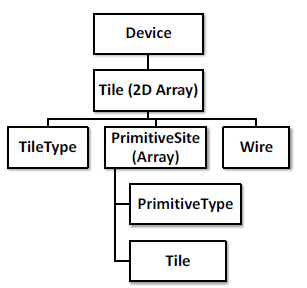
\includegraphics[height=2in]{Figures/rapidSmithDevice}
			\caption{The Device Class-Structure}
			\label{fig:rapidSmithDevice}
	\end{subfigure}%
	~ 
	\begin{subfigure}[t]{0.5\textwidth}
		\centering
		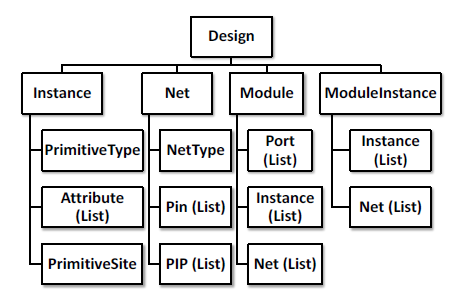
\includegraphics[height=2in]{Figures/rapidSmithDesign}
		\caption{The Design Class-Structure}
		 \label{fig:rapidSmithDesign}
	\end{subfigure}
	\caption{The \RapidSmith Class Hierarchy~\cite{rapidSmithManual}}
	 \label{fig:classStructures}
\end{figure*}
Not shown in Figure~\ref{fig:classStructures} are a series of utility classes.
The \gls{Bitstream} parser class reads and interprets the \gls{Bitstream} files. 
It uses a 'Frame' class to organize the \gls{Bitstream} file into an array of objects that adhere to the configuration pattern described in section~\ref{sec:architectureAndConfig}.
The frame objects are populated with the frame's 32-bit address, an array of 32-bit words which make up the frame and a series of helper methods.
\section{\Name}
\subsection{\acrfull{UI}}
Java and Java \Swing provide an easy to use \acrlong{UI} development system which produces light-weight, portable and cross platform applications.
The \NameNoPeriod employs \Swing to provide a very simplistic and easy to use interface which can be seen in Figure~\ref{fig:UI}.
To perform an analysis the user must use the \acrshort{UI} to navigate to and select the \gls{golden} \gls{Bitstream}, the \gls{target} \gls{Bitstream} and the \gls{golden} \acrshort{XDL} file via the three browse buttons on the left.
Once loaded the detection process can be launched via the 'Analyze' button.
On the right the user is able to review information specific to the trojan, which will be described in section~\ref{sec:operation}.
\begin{figure}
\centering
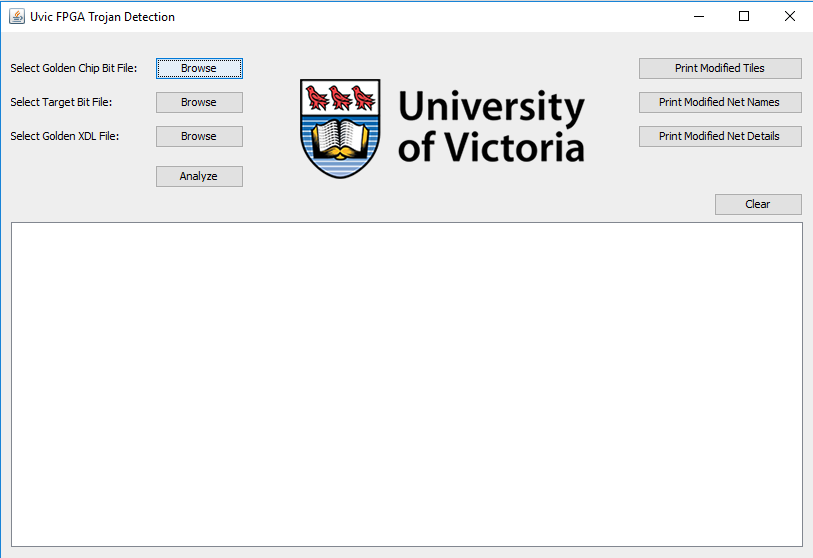
\includegraphics[width=0.96\linewidth]{Figures/UI}
\caption[The User-Interface of the \NameNoPeriod]{The User-Interface of the \NameNoPeriod}
\label{fig:UI}
\end{figure}
 
If a modification is discovered, the \NameNoPeriod analyzes it and reports a list of attributes from the taxonomy of Chapter~\ref{chapter:hardwareTrojans} which describe it.
Results are printed textually in the text window.
The attribute id-number, name, category and a brief description of the attribute are provided.
After the analysis the user is able to use the 'Print Modified Tiles' feature.
Any tile in the architecture which corresponds to a modified tile is printed to the text window. 
This provides the user with the exact location on the their device where modification took place.
The 'Print Modified Instances' feature corresponds each modified tile to the design-instance it belongs to.
\Xilinx provides schematic design views which correspond instance names to the user's design.
This can be used by the user to refer back to their design and view the trojan's effects from a high abstraction perspective.
The 'Print Modified Net Names' provides only the names of each channel that has been modified. 
Again this allows the user to relate modifications to their design.
The 'Print Modified Net Details' button provides both the names of modified nets and their corresponding list of primitives.
Finally, the 'Clear' button is a manual method of removing the text from the text-window.
\subsection{Operation} \label{sec:operation}
Figure~\ref{fig:Operation} gives a visual representation of the operating procedure of the \Name.
To perform analysis the user must submit the \gls{golden} and \gls{target} \gls{Bitstream} files.
As seen on the left of Figure~\ref{fig:Operation}, these large binary files are parsed by a utility class provided by \RapidSmith. 
The parsing utility is able to detect the model of the device by scanning the 'header' information in the files.
Different \Xilinx models use different configuration patterns.
The \gls{Bitstream} of different models may differ in a variety of features including frame size, ordering, address structure and more.
\begin{figure}[h]
	\centering
	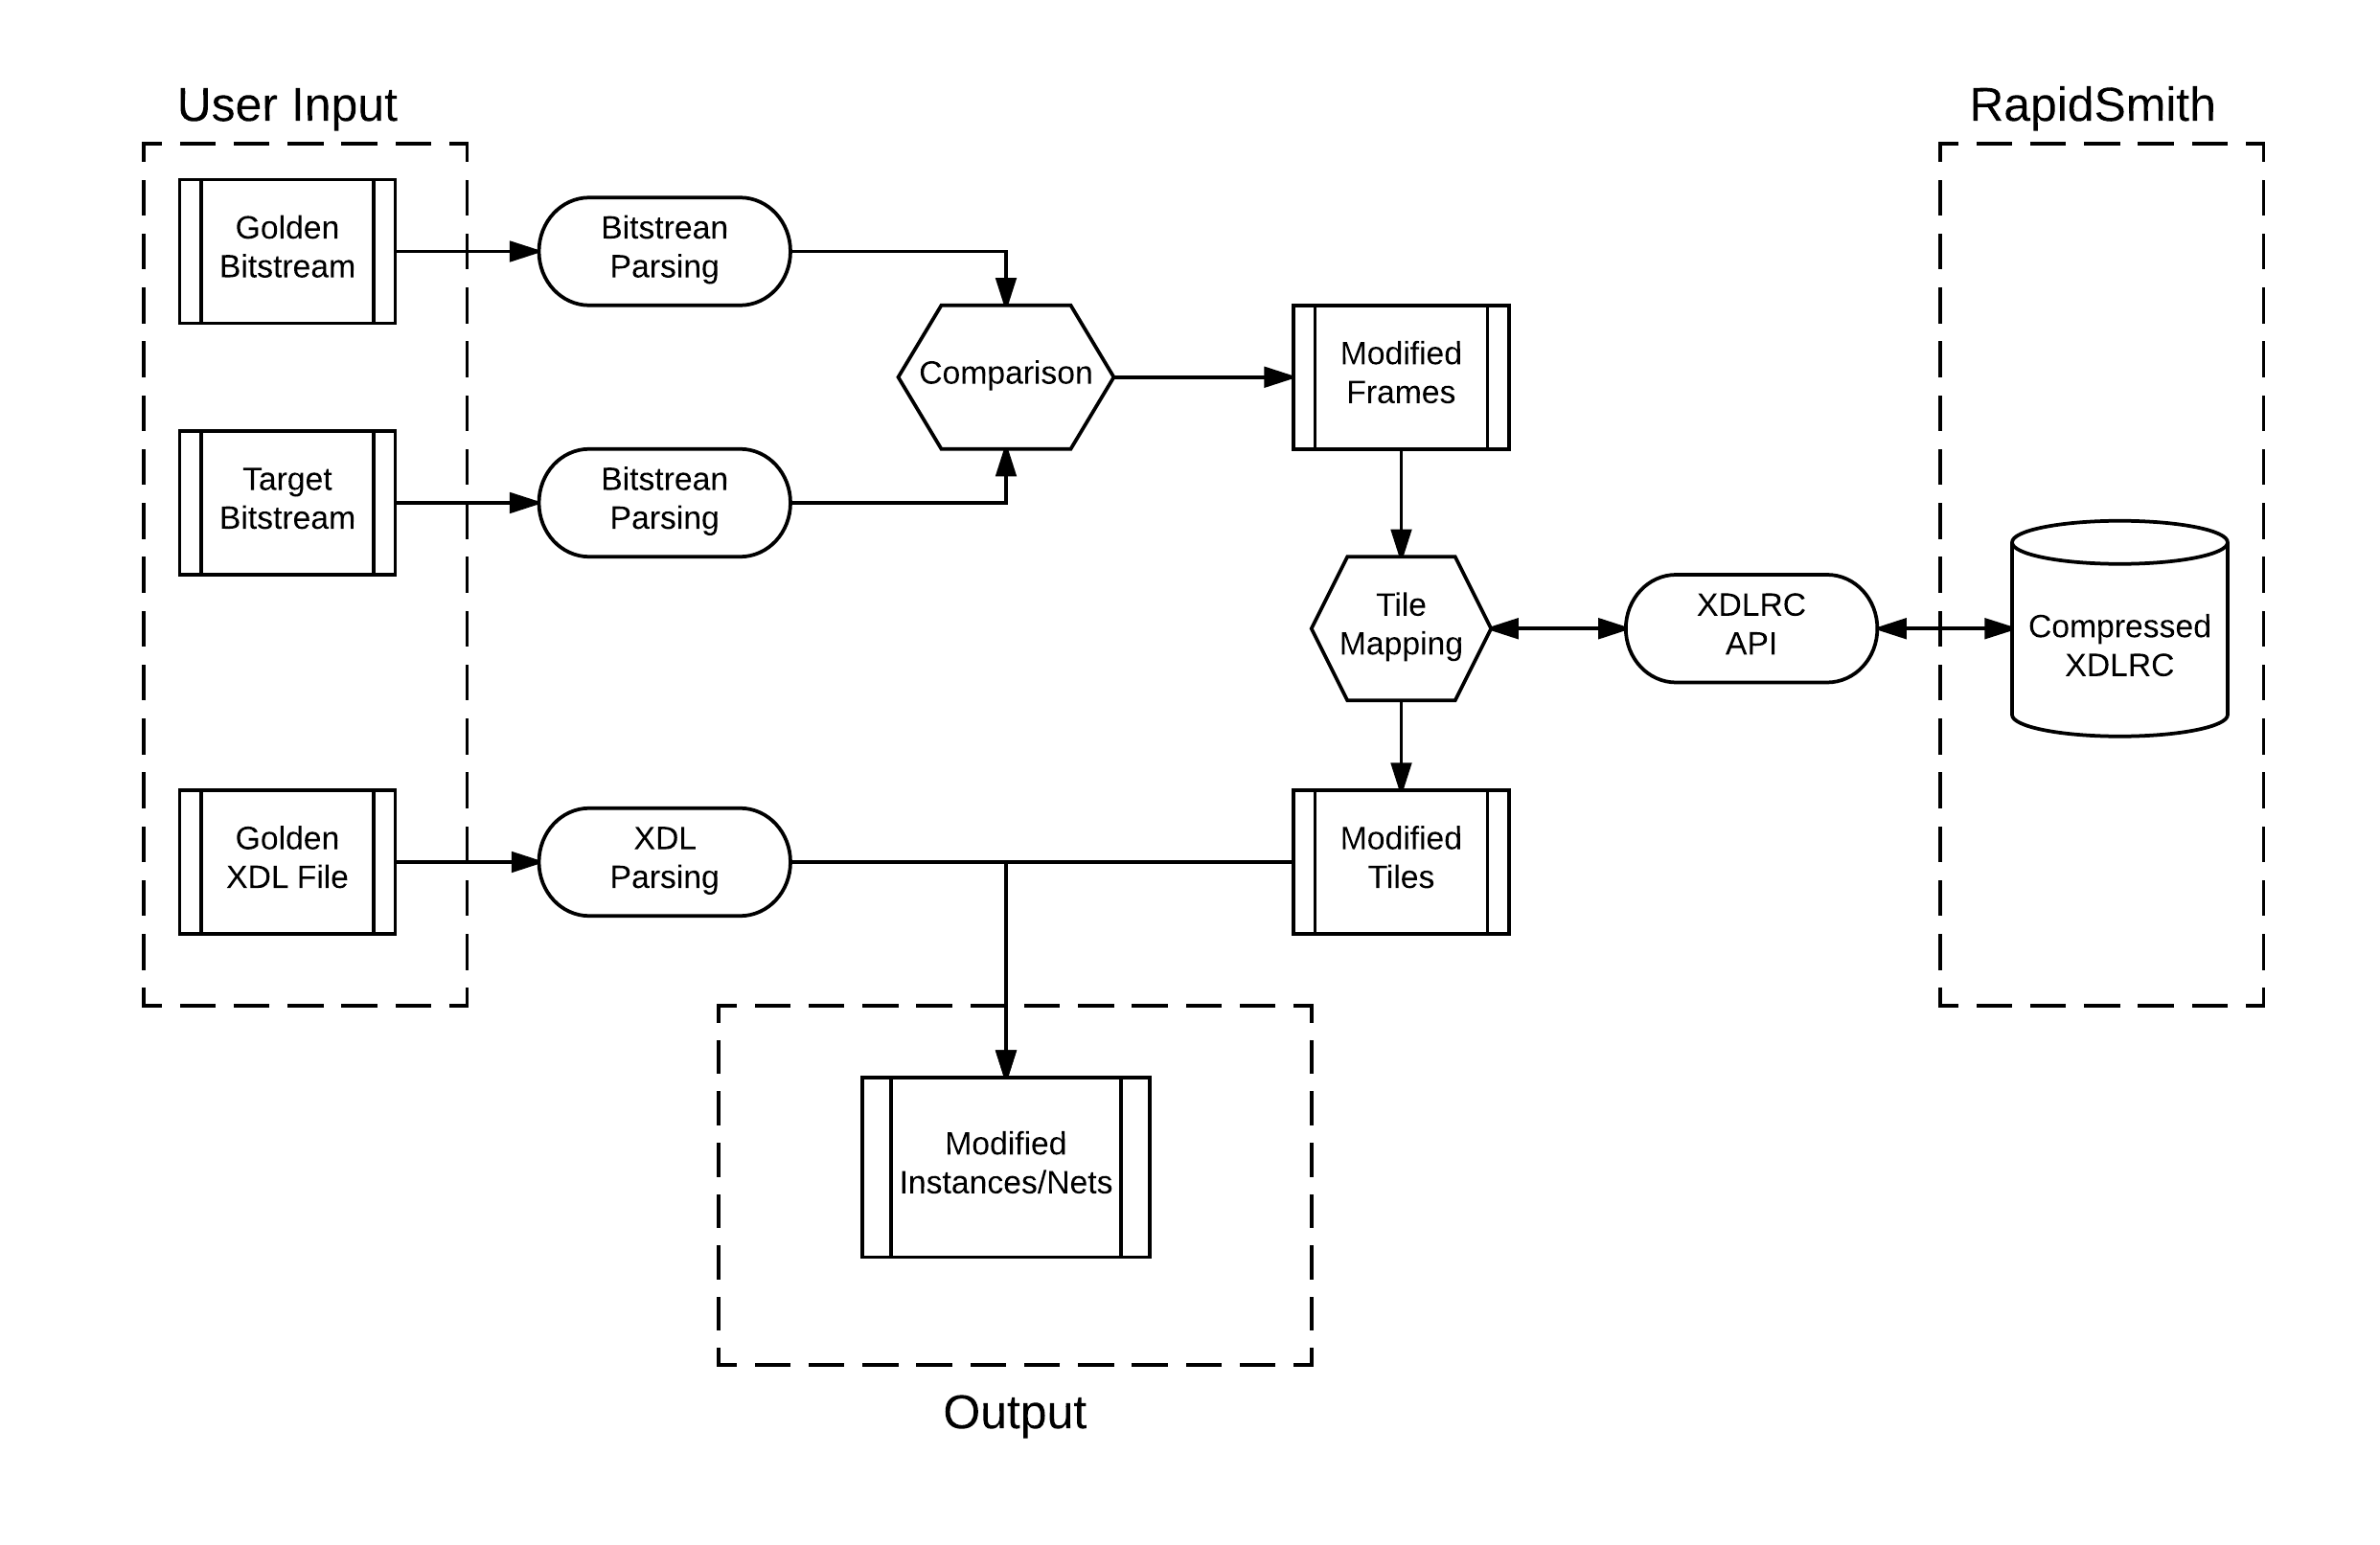
\includegraphics[width=1\linewidth]{Figures/Operation}
	\caption[Overview of Functional Operation]{Overview of Functional Operation}
	\label{fig:Operation}
\end{figure}

Knowing the device, the parser is able to refer to additional utility files and accurately extract the frames.
The \gls{golden} and \gls{target} frames are extracted and stored in memory as arrays.
The two arrays are then passed to a comparison process.
Each frame is compared bit by bit.
A trojan-free circuit will have no differences between the \gls{golden} and \gls{target} files.
Any modified frames discovered are stored in a ``Modified\_Frame'' class.
The ``Modified\_Frame'' object stores the \gls{golden} frame data, the \gls{target} frame data, the address of the frame and more.
They are then used by the 'Component Mapping' method described in section~\ref{sec:tileMapping} to determine where in the architecture the modifications have been made.

The component mapping procedure relies heavily on the compressed XDLRC files and the corresponding \acrshort{API} described in section~\ref{sec:XDLRC} as well as the ``Device'' class structure shown in Figure~\ref{fig:rapidSmithDevice}.
Component mapping produces a list of objects of the ``Modified\_Tile'' class.
This class contains a reference to the corresponding tile in the XDLRC file, the \gls{golden} and \gls{target} words (which differ), the frame address in which it occurred, the sub-column type and the column type.
The user is also required to enter the \gls{golden} \acrshort{XDL} file.
As described in section~\ref{sec:XDL} the \acrshort{XDL} file contains the Netlist for the \gls{golden} design.
This file describes not only how each of the users components are built and interconnected but where on the device they are placed.
The modified tiles, as shown in Figure~\ref{fig:Operation}, must be correlated to the users design to extract useful information.
The instances and nets described in the \acrshort{XDL} file list the exact tile and primitive in which they are placed.
The \RapidSmith \acrshort{XDL} parser reads the user's design and populates the ``Design'' class shown in Figure~\ref{fig:rapidSmithDesign}.
The list of ``Modified\_Tile'' objects are compared to the tile placings of the instances and nets in the populated ``Design'' object.
Any instances or nets that are placed in ``modified'' tiles are flagged and stored.
The user is able to view which instances and nets of their design have been modified by the four buttons on the right of the \acrshort{UI} shown in Figure~\ref{fig:UI}.

